% ================================================================== PART V
\part{Simulation, literature and conclusions}

\chapter{The CFD case: a cylinder wake at Re = 100}
Exact solutions are smooth and simple. A real application is an unsteady wake with vortices shed from a body. The project therefore simulates the 2-D laminar flow past a circular cylinder at $Re=U_\infty D/\nu=100$ in OpenFOAM, samples it in a PIV-like window, and runs the same reconstruction on that data with the CFD pressure as the reference.

The three meshes were run with the OpenFOAM v2606 MinGW build on native Windows (4 cores, MS-MPI), and the solution was inspected in ParaView 6.2 (Figure~\ref{fig:paraview}).

\section{Why this flow}
\begin{itemize}
\item Above $Re\approx47$ the steady wake becomes unstable and vortices are shed alternately from the two sides: the \textbf{K\'arm\'an vortex street}. The flow is periodic with Strouhal number $St=fD/U\approx0.165$ at $Re=100$.
\item Below $Re\approx190$ the wake stays two-dimensional (Williamson 1996), so a 2-D simulation is physically valid and planar PIV would miss nothing.
\item The shed vortices are \emph{convected} at nearly the free-stream speed while they spin more slowly: exactly the $w<c$ situation where the Lagrangian material derivative should win.
\end{itemize}

\section{Domain, mesh and boundary conditions}
\begin{figure}[H]\centering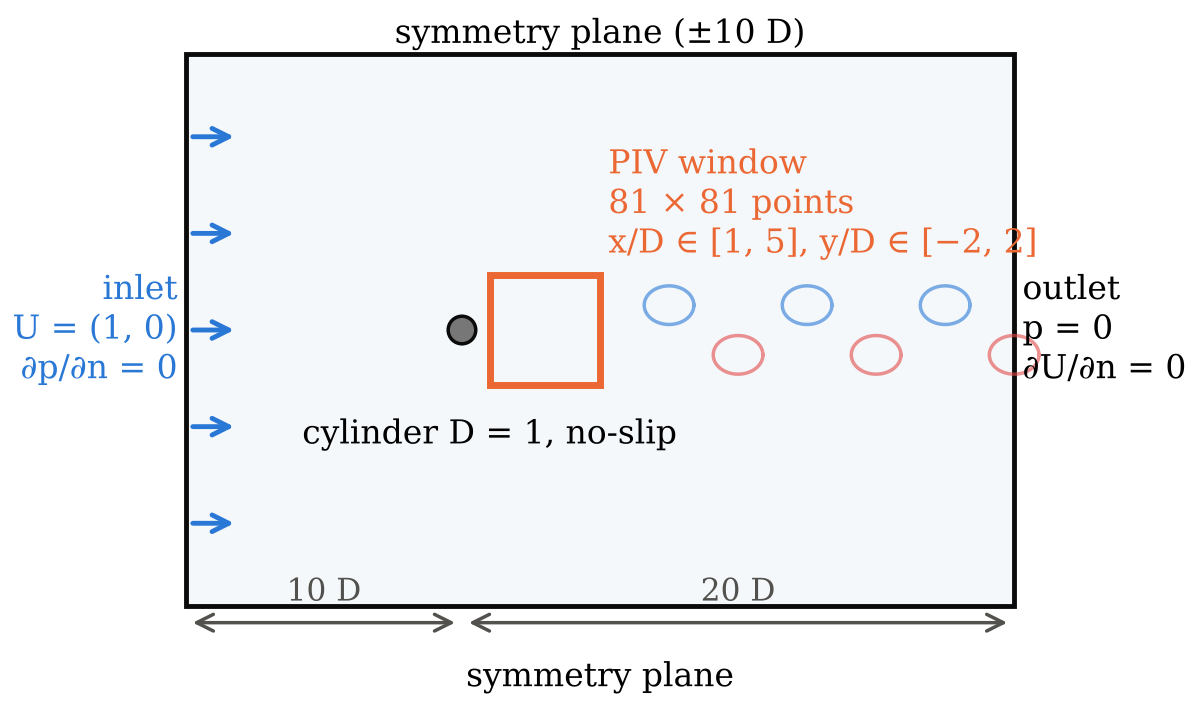
\includegraphics[width=0.62\linewidth]{img/f_cfd_domain.png}
\caption{Computational domain (not to scale), boundary conditions and the PIV sampling window.}\end{figure}

\begin{itemize}
\item \textbf{Non-dimensional set-up:} $D=1$, $U_\infty=1$, $\nu=0.01$, $\rho=1$.
\item \textbf{Domain:} 10\,$D$ upstream, 20\,$D$ downstream, $\pm10\,D$ laterally; one cell thick in $z$ with \code{empty} front and back patches (OpenFOAM's way of making a case 2-D).
\item \textbf{Boundary conditions:}
\begin{itemize}
\item inlet: $\uu=(1,0)$, $\partial p/\partial n=0$;
\item outlet: $\partial\uu/\partial n=0$, $p=0$;
\item sides: \code{symmetryPlane} (zero normal velocity and zero shear);
\item cylinder: no-slip.
\end{itemize}
\item \textbf{Blockage:} the side walls are 20\,$D$ apart, so the blockage is $D/H=5\,\%$. It slightly accelerates the flow past the cylinder and raises $C_D$ and $St$ above unbounded-domain values.
\item \textbf{Mesh:} an O-grid around the cylinder (body-fitted, near-orthogonal cells clustered radially at the wall for the boundary layer) out to the square $[-2,2]^2$, plus 8 rectangular blocks. Generated with \code{blockMesh} from a dictionary written by \code{cfd/generate\_cases.py}, which also checks the block topology.
\end{itemize}

\begin{table}[H]\centering\small
\begin{tabular}{@{}lrccc@{}}\toprule
Mesh & Cells & Cylinder tangential cell & First radial cell & Wake $\Delta y$\\\midrule
Coarse & 6\,690 & 0.033 & 0.022 & 0.167\\
Medium & 26\,760 & 0.016 & 0.011 & 0.083\\
Fine & 107\,040 & 0.008 & 0.0055 & 0.042\\\bottomrule
\end{tabular}
\caption{The three meshes: each level halves the cell size in both directions (4$\times$ the cells).}\end{table}

\section{Solver and numerics}
\begin{itemize}
\item \textbf{Solver:} \code{pimpleFoam}, laminar, run in PISO mode (\code{nOuterCorrectors 1}, \code{nCorrectors 2}, one non-orthogonal corrector).
\item \textbf{Time scheme:} \code{backward} (second-order implicit). \textbf{Convection:} \code{linearUpwind} (second-order upwind-biased).
\item \textbf{Time step:} adaptive, keeping the maximum Courant number $Co=|u|\Delta t/\Delta x\le0.5$ (with $\Delta t\le0.01$); the run goes to $t=200$, about 33 shedding periods.
\item \textbf{Start-up kick:} a perfectly symmetric mesh and inflow can delay shedding for a long time. The inlet carries $v=0.1$ for $t<5$, ramped to 0 at $t=6$; from $t=6$ on it is exactly $\uu=(1,0)$.
\end{itemize}

\textbf{How PISO works, and why it connects to this project.} In incompressible flow there is no equation \emph{for} pressure; pressure is whatever makes the velocity divergence-free. Each time step, PISO:
\begin{enumerate}
\item solves the momentum equation with the old pressure (a predicted velocity that is not divergence-free);
\item takes the divergence of the momentum equation to get a \textbf{pressure Poisson equation}, $\nabla\cdot(\tfrac1a\nabla p)=\nabla\cdot\mathbf H$, and solves it;
\item corrects the velocity and fluxes with the new pressure gradient, and repeats steps 2--3 (here two pressure correctors per step, \code{nCorrectors 2}; the pressure equation is solved with the GAMG multigrid solver).
\end{enumerate}
So the CFD solver itself recovers pressure from velocity through a Poisson equation every time step, the same mathematical step the reconstruction performs on measured data. The difference: the CFD solver has exact boundary conditions and noise-free velocity; PIV has neither.

\section{Outputs and how they are processed}
\begin{itemize}
\item \textbf{Forces:} the \code{forceCoeffs} function object writes $C_D(t)$ and $C_L(t)$ every step.
\item \textbf{PIV window:} on the fine mesh, a run-time \code{sets} function object samples $\uu$ and $p$ on an $81\times81$ grid, $x/D\in[1,5]$, $y/D\in[-2,2]$, every 0.05 time units for $t\in[175,200]$ (about 4 shedding periods). Sampling at run time avoids writing about 500 full-field dumps.
\item \code{cfd/export\_window.py} converts the samples into one array file, which the studies load as a \code{FlowField}.
\end{itemize}

\subsection{Strouhal number, drag and lift}
$C_L(t)$ is resampled on a uniform time grid (the time step is adaptive), multiplied by a Hann window (to limit spectral leakage from a non-integer number of periods), zero-padded and Fourier transformed. The peak frequency, refined by parabolic interpolation, gives $St=fD/U_\infty$. Mean $C_D$ and the $C_L$ amplitude $(\max-\min)/2$ are taken over the last 80 time units.

\subsection{Is the wake fully developed? Periodicity, not steady state}
A periodic flow never satisfies a steady-state criterion $\|\uu^{n+1}-\uu^n\|<\eps$, and its solver residuals level off instead of falling to zero (each step starts from a changed flow). The project instead cuts $C_L(t)$ into cycles at upward zero crossings and declares the flow periodic once the cycle-to-cycle changes of amplitude and period both stay below $10^{-3}$ for three consecutive cycles.

\subsection{Grid independence: Richardson extrapolation and GCI}
For a quantity $f$ (St, $\bar C_D$) on fine, medium and coarse meshes ($f_1,f_2,f_3$) with representative cell sizes $h=\sqrt{\text{area}/\text{cells}}$ and ratios $r_{21}=h_2/h_1$, $r_{32}=h_3/h_2$ (Celik et al.\ 2008):
\begin{align}
e_{21}&=f_2-f_1,\quad e_{32}=f_3-f_2,\\
p&=\frac{\big|\ln|e_{32}/e_{21}|+\ln\frac{r_{21}^p-s}{r_{32}^p-s}\big|}{\ln r_{21}},\quad s=\operatorname{sign}(e_{32}/e_{21})\quad\text{(solved by fixed-point iteration)},\\
f_{ext}&=\frac{r_{21}^pf_1-f_2}{r_{21}^p-1},\qquad
GCI_{fine}=\frac{1.25\,|e_{21}/f_1|}{r_{21}^p-1}.
\end{align}
$p$ is the observed order of accuracy (expected 1--2), $f_{ext}$ the extrapolated grid-converged value, and GCI a conservative error band on the fine-mesh value (safety factor 1.25 for three-grid studies). The asymptotic ratio $GCI_{medium}/(r_{21}^pGCI_{fine})\approx1$ confirms the meshes are in the asymptotic range.

\section{Results}

\subsection{The flow field}
\begin{figure}[H]\centering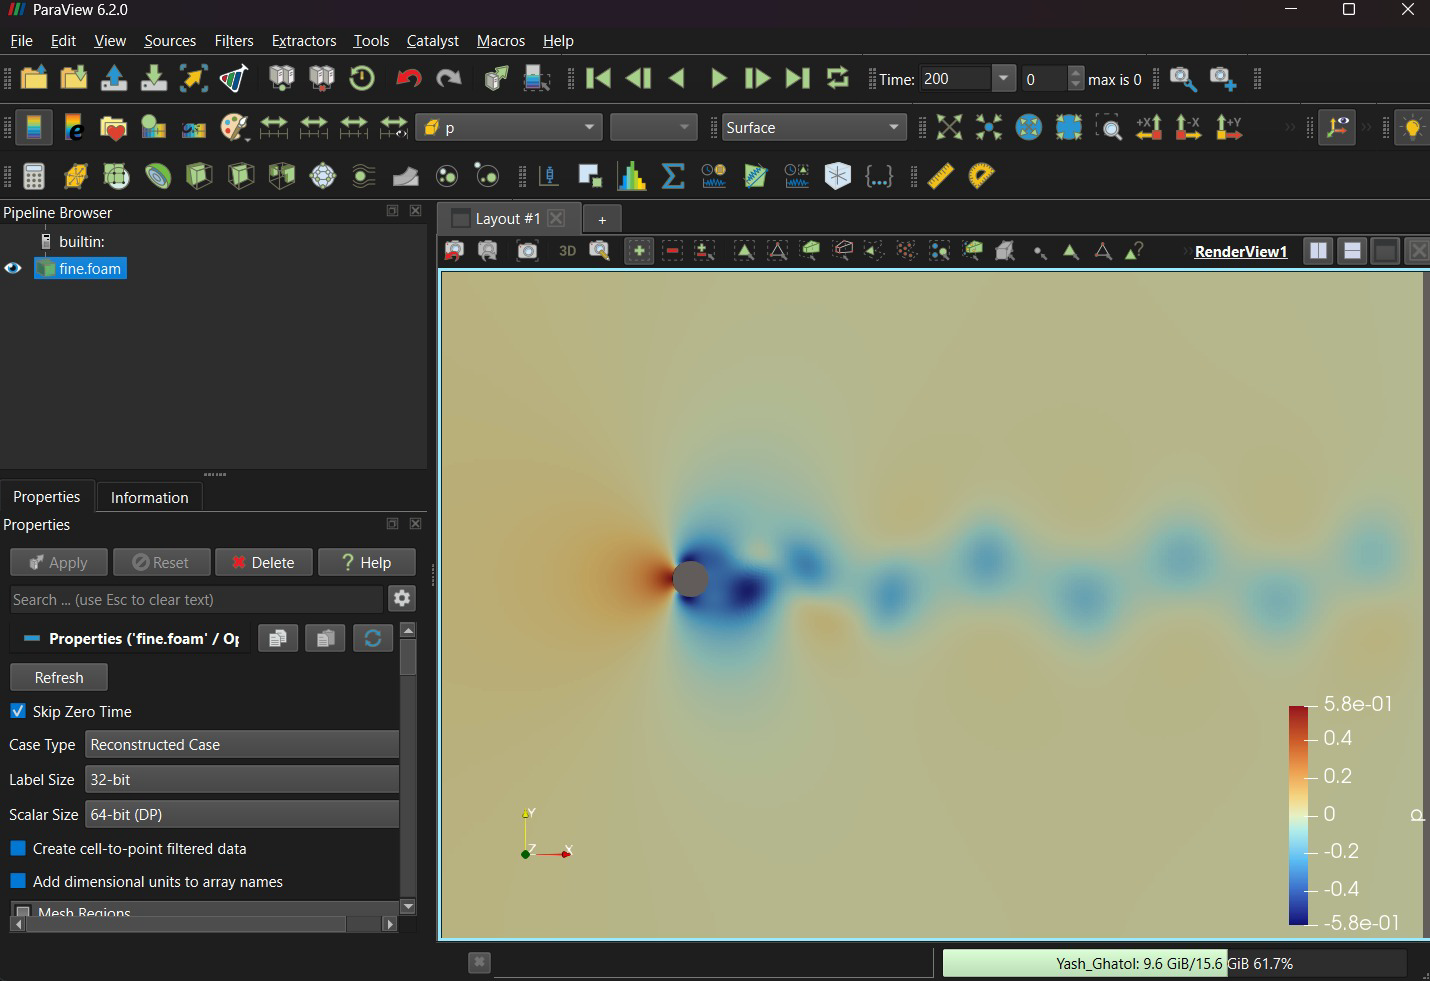
\includegraphics[width=0.9\linewidth]{img/c_paraview.png}
\caption{ParaView 6.2 screenshot (unedited) of the fine-mesh OpenFOAM solution at $t=200$, coloured by pressure. High pressure (red) at the front stagnation point, low pressure on the sides, and a K\'arm\'an street of low-pressure vortex cores alternating above and below the centreline.}\label{fig:paraview}\end{figure}

\subsection{Grid independence}
\begin{table}[H]\centering\small
\begin{tabular}{@{}lrccc@{}}\toprule
Mesh & Cells & $St$ & $\bar C_D$ & $C_L$ amplitude\\\midrule
Coarse & 6\,690 & 0.1644 & 1.3754 & 0.3216\\
Medium & 26\,760 & 0.1688 & 1.3880 & 0.3451\\
\textbf{Fine} & \textbf{107\,040} & \textbf{0.1695} & \textbf{1.3879} & \textbf{0.3451}\\
Richardson extrapolation & -- & 0.1697 & converged & converged\\\midrule
2-D simulations, Re = 100 (approx.) & -- & 0.164--0.165 & $\approx1.33$ & $\approx0.33$\\\bottomrule
\end{tabular}
\caption{Grid independence (analysis window: last 80 time units, 13--14 shedding periods per mesh; amplitude drift $\le0.04\,\%$).}\end{table}

\begin{table}[H]\centering\footnotesize\setlength{\tabcolsep}{4pt}
\begin{tabular}{@{}lccccccc@{}}\toprule
Quantity & coarse$\to$medium & medium$\to$fine & $p$ & $f_{ext}$ & GCI$_{medium}$ & GCI$_{fine}$ & asympt.\ ratio\\\midrule
$St$ & 2.67\,\% & 0.46\,\% & 2.48 & 0.1697 & 0.71\,\% & 0.13\,\% & 1.005\\
$\bar C_D$ & 0.91\,\% & 0.00\,\% & -- & -- & -- & -- & --\\
$C_L$ amplitude & 7.30\,\% & 0.01\,\% & -- & -- & -- & -- & --\\\bottomrule
\end{tabular}
\caption{Richardson extrapolation and grid convergence index, from \code{grid\_independence.md}.}\end{table}

\begin{figure}[H]\centering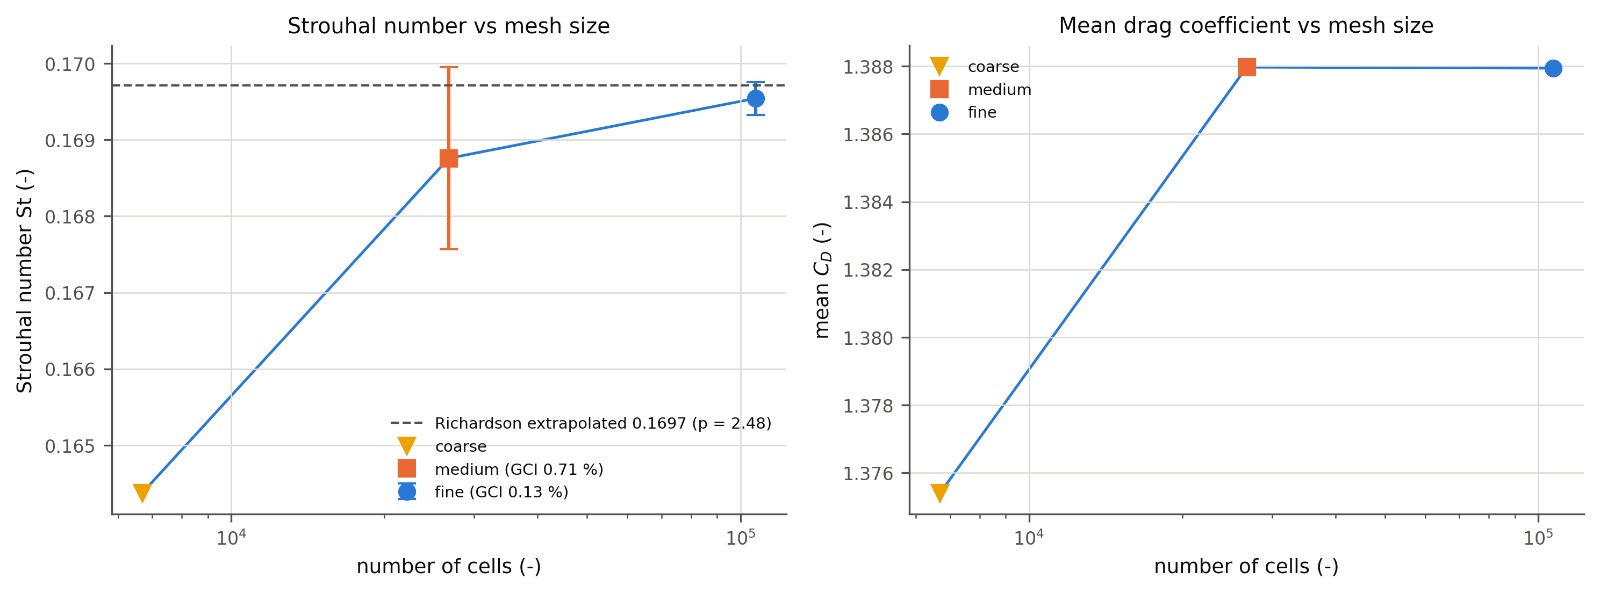
\includegraphics[width=\linewidth]{img/c_st.png}
\caption{Strouhal number and mean drag vs number of cells; error bars on St are the GCI; dashed line the Richardson-extrapolated value.}\end{figure}

\begin{itemize}
\item \textbf{St converges monotonically}: the change falls from 2.67\,\% to 0.46\,\% per refinement. The observed order $p=2.48$ is close to the nominal second order of the schemes, the extrapolated value is 0.1697 and the fine-mesh GCI is 0.13\,\%. The asymptotic ratio 1.005 ($\approx1$) shows the three meshes are in the asymptotic range.
\item \textbf{Mean drag and lift amplitude converge already on the medium mesh} (changes 0.00\,\% and 0.01\,\%). With $e_{21}\approx0$ the observed order is undefined (the ratio $e_{32}/e_{21}$ blows up), so no Richardson value is reported: the medium--fine difference is below the resolution of the time averaging.
\item The \textbf{coarse mesh} under-predicts both St and the lift amplitude (0.322 vs 0.345): with a 0.022\,$D$ first cell it under-resolves the boundary layer and the separation.
\end{itemize}

\begin{figure}[H]\centering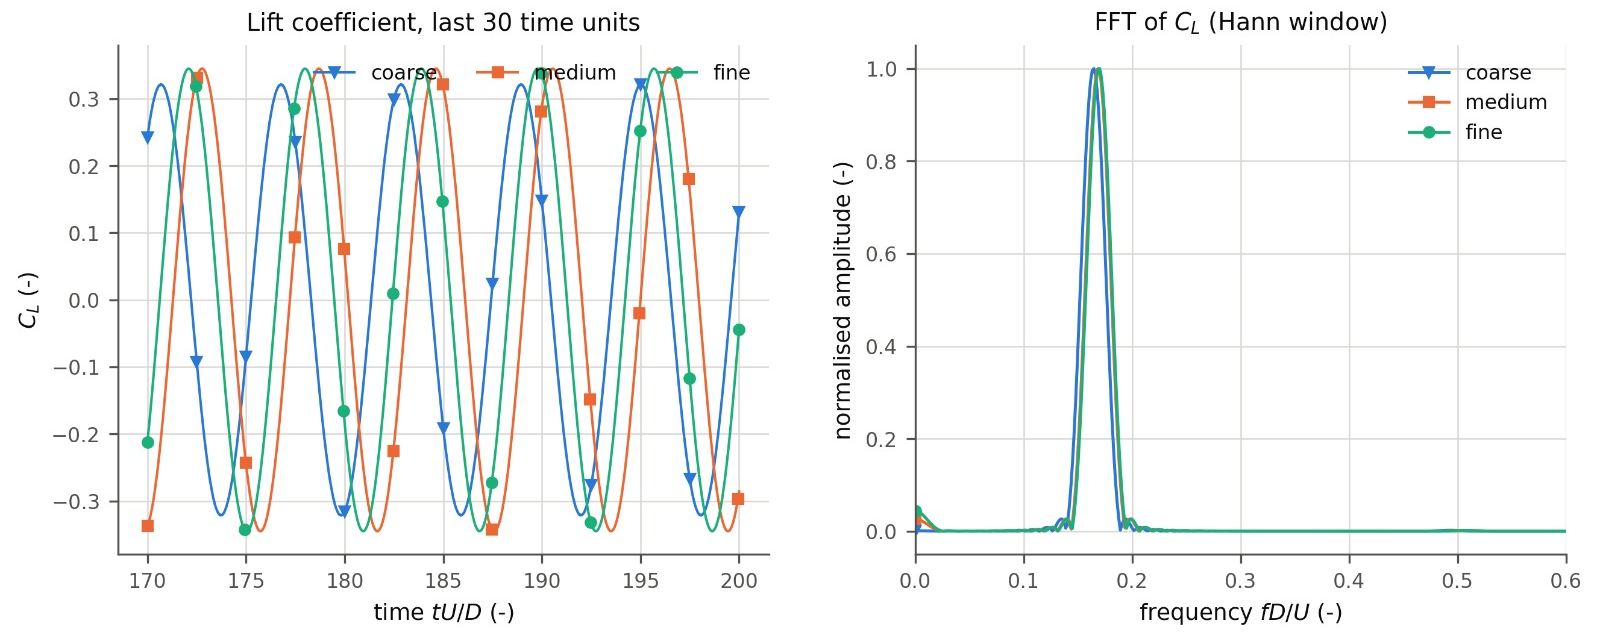
\includegraphics[width=\linewidth]{img/c_clfft.png}
\caption{Lift coefficient over the last 30 time units for the three meshes, and its spectrum (Hann window). The single sharp peak at $fD/U\approx0.17$ is the shedding frequency.}\end{figure}

\subsection{Residuals and periodicity}
\begin{figure}[H]\centering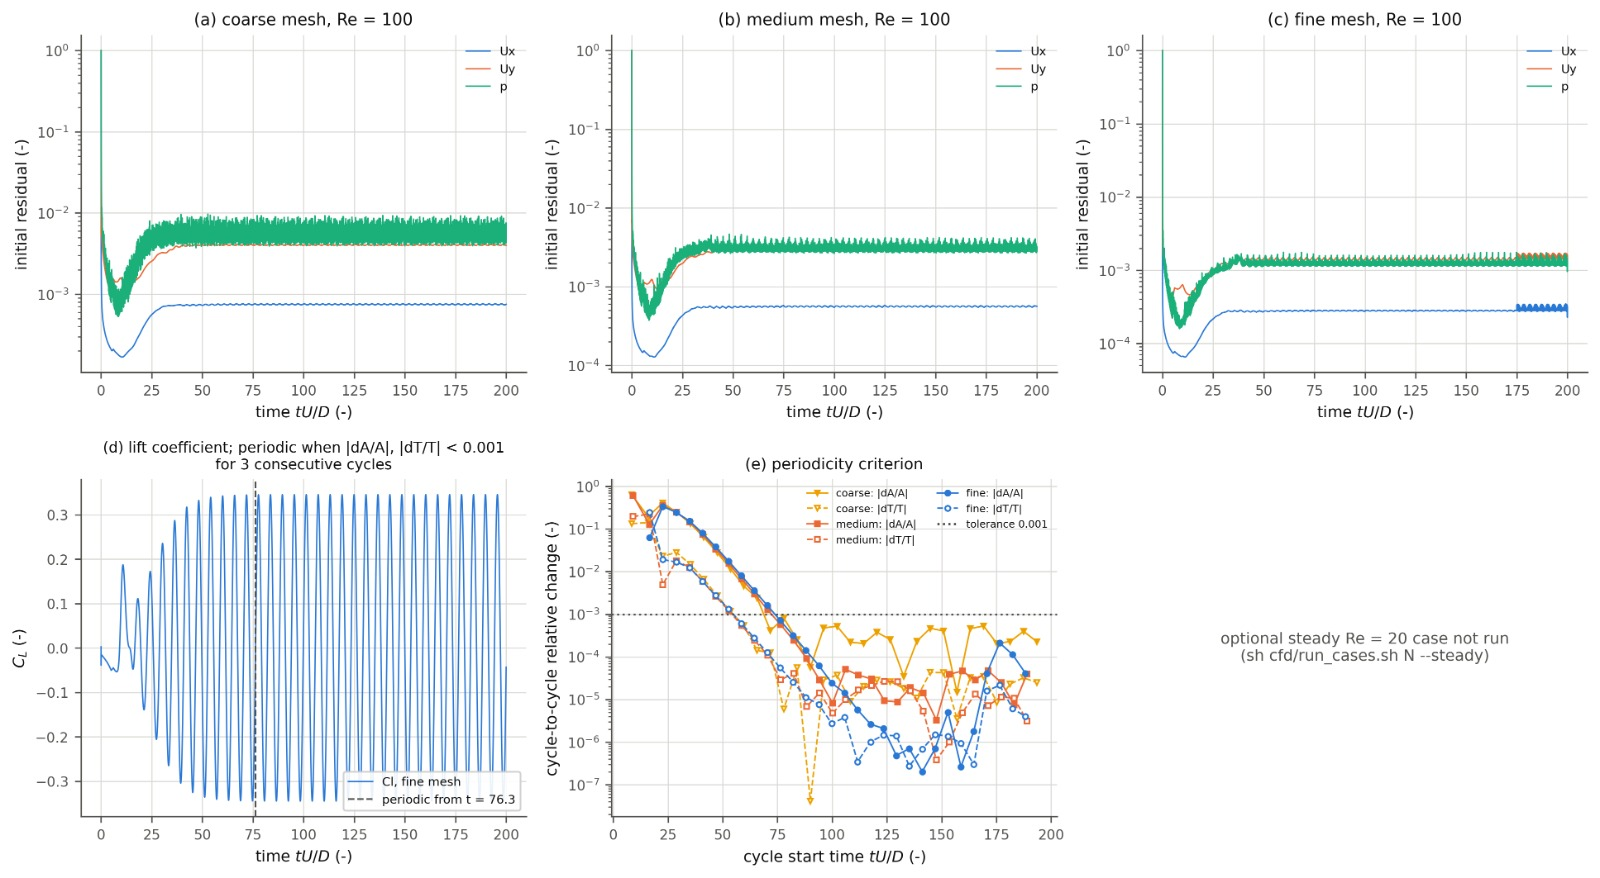
\includegraphics[width=\linewidth]{img/c_resid.png}
\caption{(a)--(c) Initial residuals of $U_x$, $U_y$ and $p$ for the three meshes; (d) fine-mesh lift, periodic from $t=76.3$; (e) cycle-to-cycle relative change of the lift amplitude and period.}\end{figure}
\begin{itemize}
\item \textbf{Residuals level off} (fine mesh: about $10^{-3}$ for $p$ and $U_y$, $3\times10^{-4}$ for $U_x$) instead of falling to zero. This is expected for a periodic flow: every time step starts from a changed flow (Section~12.4.2). Finer meshes level off lower. The small step on the fine mesh after $t=175$ coincides with the start of window sampling, which also caps the time step to hit the sample times.
\item \textbf{The wake is periodic from $t=76.3$} on the fine mesh: the cycle-to-cycle change of amplitude and period stays below $10^{-3}$. The PIV window ($t=175$--200) is therefore fully developed. The coarse mesh hovers around the tolerance, another sign of under-resolution.
\end{itemize}

\subsection{Pressure reconstructed from the CFD velocity}
\begin{figure}[H]\centering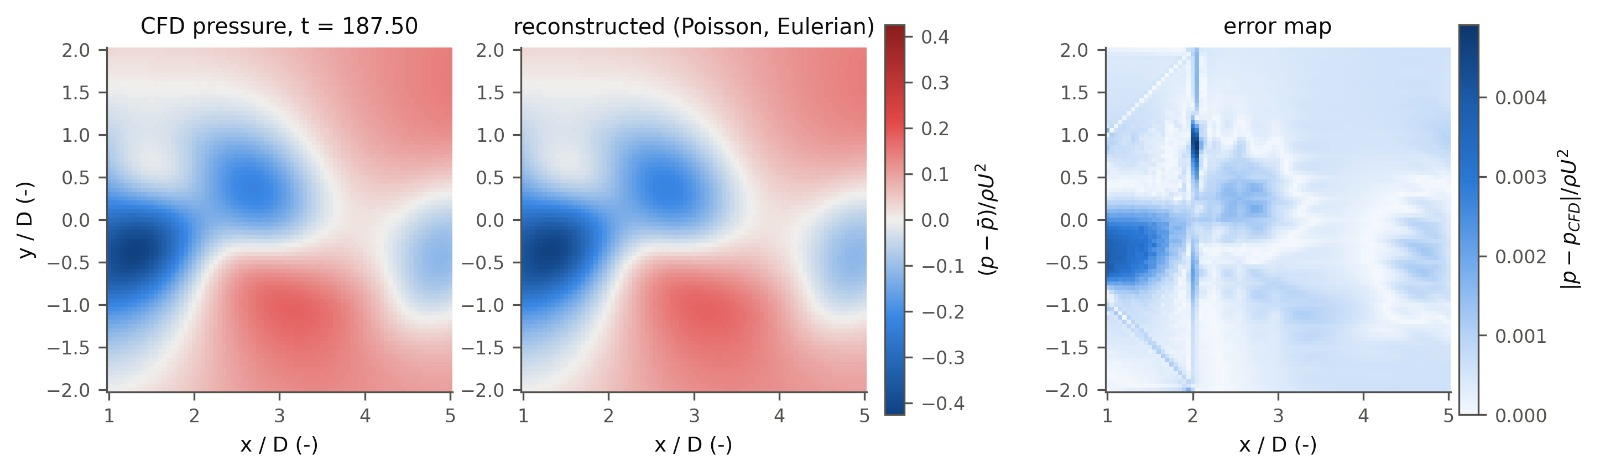
\includegraphics[width=\linewidth]{img/c_fields.png}
\caption{At $t=187.5$: CFD pressure in the window, pressure reconstructed from the CFD velocity samples (Poisson, Eulerian, no noise, $h=0.05D$), and the error map.}\end{figure}
\begin{figure}[H]\centering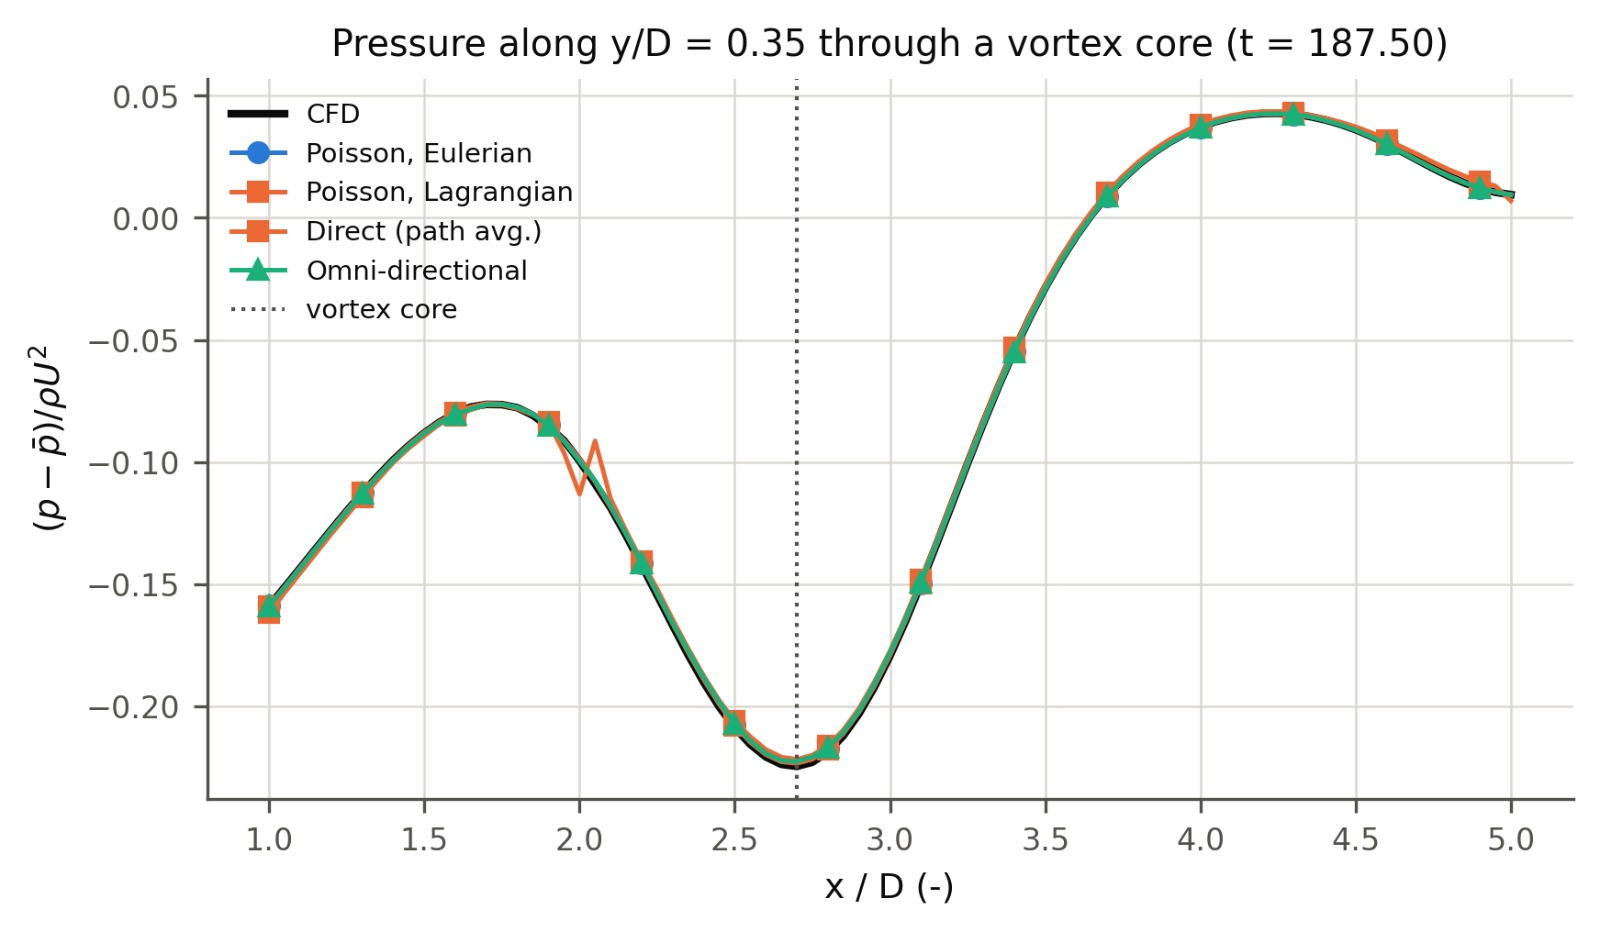
\includegraphics[width=0.75\linewidth]{img/c_line.png}
\caption{Pressure along $y/D=0.35$, through a shed vortex core: CFD and four reconstructions.}\end{figure}

\begin{enumerate}
\item \textbf{The wake pressure is recovered}: without noise the Poisson error is $\eps_{L2}=0.5$--0.75\,\% over a shedding period. All methods reproduce the vortex-core suction ($-0.22\rho U^2$ at $x/D\approx2.7$) within about 1\,\%.
\item \textbf{The error lies on the CFD mesh's block boundaries}: the vertical line $x/D=2$ and the diagonals towards $(2,\pm2)$ are exactly the edges of the O-grid around the cylinder, which extends to the square $[-2,2]^2$. The sampled velocity (interpolated from cell values) has small slope discontinuities across these block edges, where cell size and orientation change; differentiation turns these kinks into steps in $\G$. Direct integration, which carries every error along its path, shows a visible kink at $x/D=2$. This is a systematic error of the ``measured'' data, analogous to a calibration error in real PIV, and it is amplified by exactly the mechanism of Chapter~4.
\item \textbf{The largest error is near the inflow edge of the window} ($x/D\approx1$--1.7, $y<0$), where a new vortex is forming close to the cylinder and gradients are steepest.
\end{enumerate}

\subsection{Time step, scheme and noise on the wake}
\begin{figure}[H]\centering
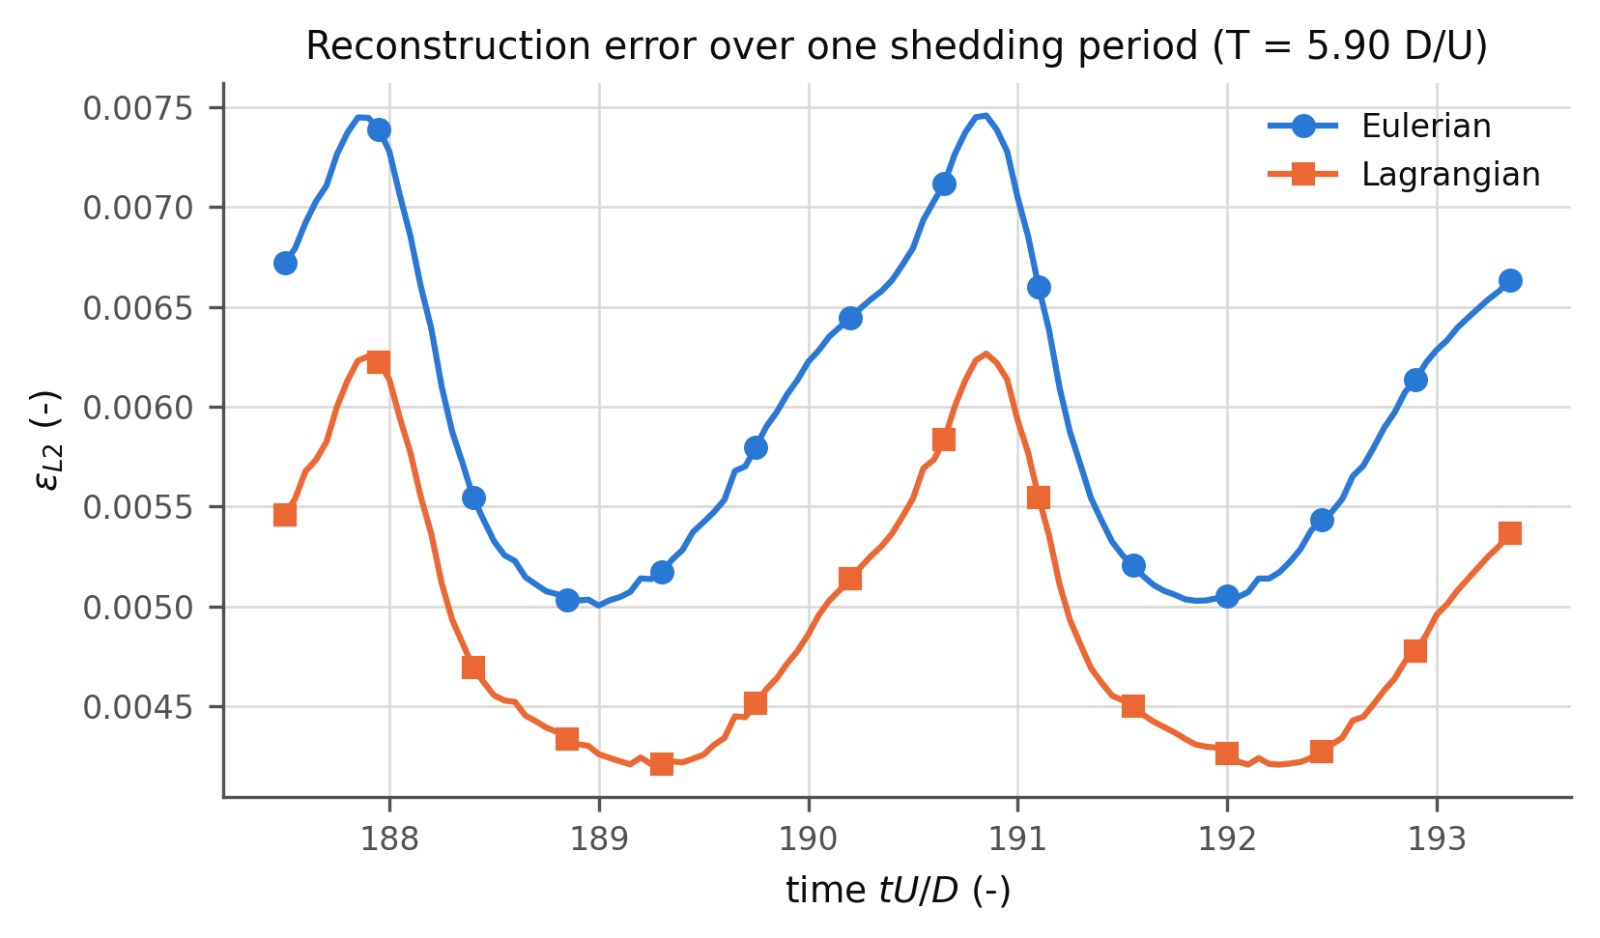
\includegraphics[width=0.62\linewidth]{img/c_period.png}\hfill
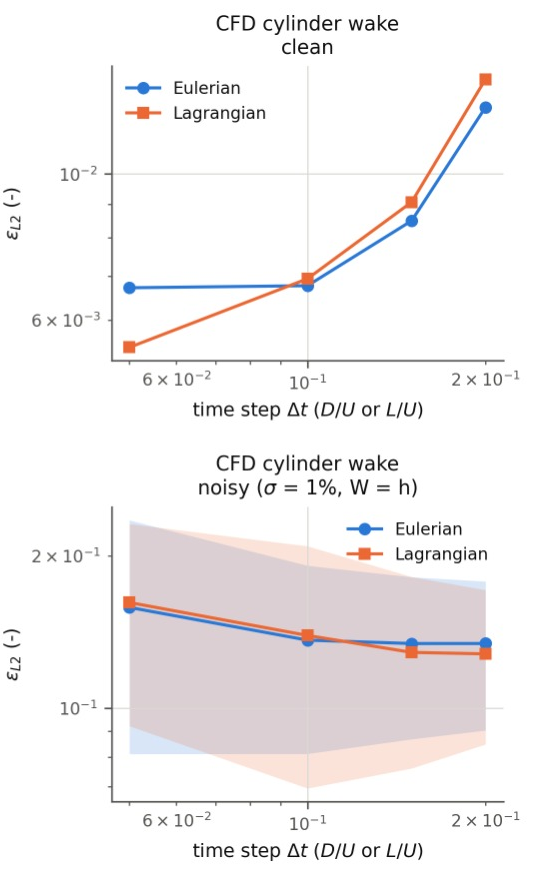
\includegraphics[width=0.3\linewidth]{img/c_dt_cfd.png}
\caption{Left: reconstruction error over one shedding period ($T=5.90$, clean, $\Delta t=0.05$). Right: error vs time step on the wake, clean (top) and with $\sigma=1\,\%$ noise (bottom).}\end{figure}

\begin{enumerate}
\item \textbf{The error pulses twice per shedding period} ($T=5.90$, so $St=1/T=0.1695$, consistent with the FFT). Each peak occurs as a new vortex forms on one side of the cylinder, near the inflow edge of the window.
\item \textbf{At $\Delta t=0.05$ the Lagrangian scheme is 15--18\,\% better} throughout the period ($\eps\approx0.0042$--0.0063 vs 0.0050--0.0075), as predicted for structures carried through the window.
\item \textbf{At $\Delta t\ge0.1$ the Eulerian scheme is slightly better} (e.g.\ $8.4\times10^{-3}$ vs $9.1\times10^{-3}$ at $\Delta t=0.15$), unlike the convected Taylor--Green vortex. The theory of Section~3.2 assumes a pattern simply carried along ($w\ll c$). In the near wake ($x/D=1$--5) the vortices are still forming: they move slower than $U_\infty$ and rotate quickly ($w$ comparable to $c$), so particle paths curve strongly and the straight-line tracking error grows quickly with $\Delta t$. More tracked points also leave the $4D\times4D$ window at larger $\Delta t$ and fall back to the Eulerian estimate. Both are plausible contributors; separating them would need the fallback fraction and a longer window.
\item \textbf{With 1\,\% noise} the error is $\eps\approx0.13$--0.15 for both schemes and almost flat in $\Delta t$: noise amplification dominates truncation. It is larger than on Taylor--Green (0.08) because the wake's pressure variations are only about $\pm0.2\rho U^2$, so the same velocity noise is larger relative to the signal.
\end{enumerate}

\begin{keyidea}[What the CFD case adds]
The analytic tests isolate each error source; the wake combines them on a realistic unsteady flow. The reconstruction recovers the wake pressure to better than 1\,\% from clean data, the Lagrangian advantage holds only at small $\Delta t$ in the vortex-formation region, and systematic kinks in the data (here from the CFD mesh) are amplified just like random noise.
\end{keyidea}

% ------------------------------------------------------------------
\chapter{Comparison with published studies}
The project's controlled synthetic experiments can be checked against the conclusions of the PIV-pressure literature.

\begin{table}[H]\centering\small
\begin{tabularx}{\linewidth}{@{}>{\raggedright\arraybackslash}X>{\raggedright\arraybackslash}Xl@{}}\toprule
This project & Published finding & Match\\\midrule
Exact $p$ on 2 edges: $\eps$ 0.044 vs 0.082 all-Neumann ($\approx2\times$) & Pan et al.\ (2016): Dirichlet boundaries give less error than Neumann (about 2$\times$ for large domains with boundary error); avoid pure Neumann where possible & Agrees\\
Bernoulli edges: $\eps$ 0.30--0.81 in rotational flow & Pan et al.\ (2016): Bernoulli-based Dirichlet data are valid only in irrotational regions & Agrees\\
Errors from 0.002\,\% (clean, fine) to $>100$\,\% (direct, $\sigma\ge2\,\%$); depend on method, spacing, filtering & Charonko et al.\ (2010), as summarised by Pan et al.: errors from $<1\,\%$ to $>100\,\%$, sensitive to all these factors, no single best method & Agrees\\
Lagrangian 3$\times$ better at large $\Delta t$ in convected flow; noise $\propto1/\Delta t$ & Violato et al.\ (2011): the Eulerian approach is limited to short $\Delta t$; short $\Delta t$ amplifies precision error, long $\Delta t$ adds truncation error & Agrees\\
Omni and Poisson recover the main features; direct integration very noise-sensitive & van Gent et al.\ (2017): all methods tested recover the main features; noise lowers accuracy but no method was critically sensitive at their noise levels & Partly\\
Cylinder wake (fine mesh): $St=0.1695$, $\bar C_D=1.388$, $C_L$ amplitude 0.345 & 2-D simulations at Re = 100 (e.g.\ Park et al.\ 1998): $St\approx0.164$--0.165, $\bar C_D\approx1.33$; experiments $St\approx0.164$ (Williamson 1996) & Agrees\\\bottomrule
\end{tabularx}\end{table}

\textbf{Why ``partly'' for van Gent et al.} Their comparison used tomographic PIV and Lagrangian particle tracking data with more advanced methods (least-squares pseudo-tracking, vortex-in-cell, FlowFit); simple single-path direct integration was not among them. Our direct-integration result does not contradict them, it covers a method they did not test.

\textbf{Why the wake values are 3--4\,\% high.} The $\pm10D$ symmetry sides block 5\,\% of the channel. The flow accelerates past the cylinder, which raises the drag and the shedding frequency; a few per cent is a plausible size for 5\,\% blockage, though we did not run a wider domain to confirm it. The literature values are for (nearly) unbounded domains and are quoted approximately; confirm them in the papers before quoting exact numbers.

\textbf{What the literature adds that we did not test.} Pan et al.\ show that the error also depends on the domain size and shape (for Dirichlet domains of fixed area, a square is the worst case). Our windows are all square, so this is a natural next study.

% ------------------------------------------------------------------
\chapter{Conclusions}

\section{Key findings}
\begin{enumerate}
\item \textbf{The code is verified.} All three algorithms are second-order accurate on exact Navier--Stokes solutions (slopes 1.8--2.1), including the boundaries.
\item \textbf{Noise, not discretisation, limits PIV pressure.} The error grows linearly with the velocity noise, and there is an optimum vector spacing ($h\approx0.03$ here) below which noise amplification by the derivatives dominates.
\item \textbf{The integration method matters.} Poisson and omni-directional integration are 5--7$\times$ more robust than direct integration because they average errors over many paths; Poisson is about 27$\times$ faster than omni.
\item \textbf{Boundary data matter.} Known pressure on two opposite edges halves the error; Bernoulli edges are valid only in irrotational flow; with pure Neumann data, a zero-mean constraint beats pinning a node.
\item \textbf{The time step is a trade-off.} The Lagrangian material derivative tolerates larger $\Delta t$ in convected flow; with noisy data a larger $\Delta t$ helps both schemes.
\item \textbf{Smoothing trades noise for bias.} Denoising cuts the noisy error about 3$\times$ but hurts clean data.
\item \textbf{The CFD wake.} The OpenFOAM solution is grid-independent (St = 0.1695, GCI 0.13\,\%) and periodic from $t=76$. From its velocity the pressure is reconstructed to 0.5--0.75\,\%; the remaining error sits on the CFD mesh's block edges, where kinks in the data are amplified like noise. The Lagrangian advantage holds only at small $\Delta t$ in the near wake.
\item \textbf{Solvers.} SOR (at the Neumann-corrected $\omega_{opt}$) and CG need 80--140$\times$ fewer iterations than Jacobi; classic Jacobi stalls on the all-Neumann problem; a small change per iteration is not proof of convergence.
\end{enumerate}

\section{Objectives}
All four objectives are met: the algorithms are implemented, verified on exact flows, studied parametrically, and compared with a CFD simulation and with published studies.

\begin{keyidea}[Main takeaway]
PIV pressure is limited by how velocity noise is amplified by differentiation. The choice of method, boundary data, vector spacing and time separation decides whether that noise is averaged out or accumulated.
\end{keyidea}

\section{Recommended practice}
Use a Poisson solver; impose Dirichlet values only where pressure is genuinely known (taps, free stream); use the Lagrangian material derivative with the largest $\Delta t$ that keeps truncation error small; choose the vector spacing near the noise--truncation optimum rather than the finest possible; apply light denoising above $\sigma\approx0.5\,\%$.

\section{Limitations and future work}
\begin{itemize}
\item \textbf{Noise model:} $\sigma$ is independent of the window size and uncorrelated between neighbouring vectors. Real PIV has less random error for larger windows and spatially correlated errors from overlapping windows.
\item \textbf{Two-dimensional data:} planar PIV of 3-D turbulence misses $-\rho w\,\partial\uu/\partial z+\mu\,\partial^2\uu/\partial z^2$, an $O(1)$ error that refinement cannot remove. The project includes a loader and out-of-plane term calculator for turbulence-database slices (JHTDB) but no data were analysed.
\item \textbf{Omni-directional method:} a rotating-ray variant of Liu \& Katz (2006), not a line-by-line copy.
\item \textbf{Domain shape:} only square windows were tested.
\item \textbf{CFD window:} the $4D\times4D$ window sits in the vortex-formation region and crosses mesh block edges; a window further downstream on a uniform-mesh region would separate the two effects.
\item \textbf{Next steps:} window-dependent noise; correlated noise; a downstream CFD window; 3-D time-resolved data.
\end{itemize}
